\documentclass[11pt]{article}
\usepackage[margin=1in]{geometry}
\usepackage{amsmath, amssymb}
\usepackage{graphicx}
\usepackage{array}
\usepackage{tabularx}
\usepackage{booktabs}
\usepackage{enumitem}
\usepackage{hyperref}
\usepackage{caption}
\usepackage{titlesec}
\usepackage{graphicx}
\usepackage{float} % for [H]
\titleformat{\section}{\large\bfseries}{\thesection.}{1em}{}

\begin{document}

\begin{center}
    \Large \textbf{Sri Sivasubramaniya Nadar College of Engineering, Chennai} \\
    \large (An autonomous Institution affiliated to Anna University) \\
    \vspace{0.3cm}
\end{center}
\begin{table}[h]
\renewcommand{\arraystretch}{1.4}
\resizebox{\textwidth}{!}{%
\begin{tabular}{|l|l|l|l|}
\hline
Degree \& Branch & B.E. Computer Science \& Engineering & Semester & VI \\ \hline
Subject Code \& Name & \multicolumn{3}{l|}{UCS2612 – Machine Learning Algorithms Laboratory} \\ \hline
Academic Year & 2025–2026 (Even) & Batch & 2023–2027 \\ \hline
Name & Munish Madhav M & Register No. & 3122235001086 \\ \hline
Due Date & \multicolumn{3}{l|}{07.03.2026} \\ \hline
\end{tabular}}
\end{table}
\begin{center}
    \textbf{Experiment 9: Clustering Human Activity Recognition Data using K-Means, DBSCAN, and Hierarchical Clustering}
\end{center}

\section*{Objective}
To implement and analyze the performance of clustering algorithms on the Human Activity Recognition dataset:
\begin{itemize}
    \item \textbf{Model A:} K-Means Clustering.
    \item \textbf{Model B:} DBSCAN (Density-Based Spatial Clustering of Applications with Noise).
    \item \textbf{Model C:} Hierarchical Agglomerative Clustering (HAC).
\end{itemize}
Students must visualize and compare the clusters formed by each algorithm, report results, and analyze performance.

\section*{Dataset}
\textbf{Download:} \href{https://archive.ics.uci.edu/dataset/240/human+activity+recognition+using+smartphones}{Human Activity Recognition Using Smartphones Dataset}  

- 30 volunteers (aged 19–48).  
- 6 activities: WALKING, WALKING\_UPSTAIRS, WALKING\_DOWNSTAIRS, SITTING, STANDING, LAYING.  
- Sensors: 3-axis accelerometer and gyroscope (50 Hz).  
- Preprocessed into windows of 2.56s (128 readings/window) with feature extraction from time and frequency domain.  

\section*{Theory}
\subsection*{K-Means Clustering}
- Objective: Partition data into $k$ clusters by minimizing within-cluster variance.  
- Distance metric: Euclidean.  
- Algorithm:
\begin{enumerate}
    \item Initialize $k$ centroids.
    \item Assign points to nearest centroid.
    \item Update centroids as mean of assigned points.
    \item Repeat until convergence.
\end{enumerate}

\subsection*{Elbow Method for Choosing $k$}
- Compute \textbf{Within-Cluster Sum of Squares (WCSS)} for different $k$ values.  
- Plot $k$ vs. WCSS.  
- The ``elbow point'' (where reduction in WCSS slows down) suggests the optimal $k$.  

\begin{table}[H]
\centering
\caption{K-Means Elbow Method Results}
\renewcommand{\arraystretch}{1.3}
\begin{tabular}{|c|c|c|}
\hline
\textbf{Number of Clusters ($k$)} & \textbf{WCSS (Inertia)} & \textbf{Silhouette Score} \\
\hline
2 & 918351 & 0.3921 \\
3 & 814303 & 0.3039 \\
4 & 777281 & 0.1353 \\
5 & 750010 & 0.1079 \\
6 & 729516 & 0.1030 \\
7 & 711693 & 0.1050 \\
8 & 697957 & 0.1012 \\
\hline
\end{tabular}
\end{table}
\vspace{0.3cm}
\noindent\textbf{Justification for k=6:} Based on the Elbow Curve, the rate of decrease in WCSS (inertia) slows down noticeably around k=6, forming an ``elbow.'' Additionally, k=6 perfectly aligns with the domain knowledge of the dataset, which contains exactly 6 distinct human activities.
\vspace{0.3cm}
\begin{figure}[H]
    \centering
    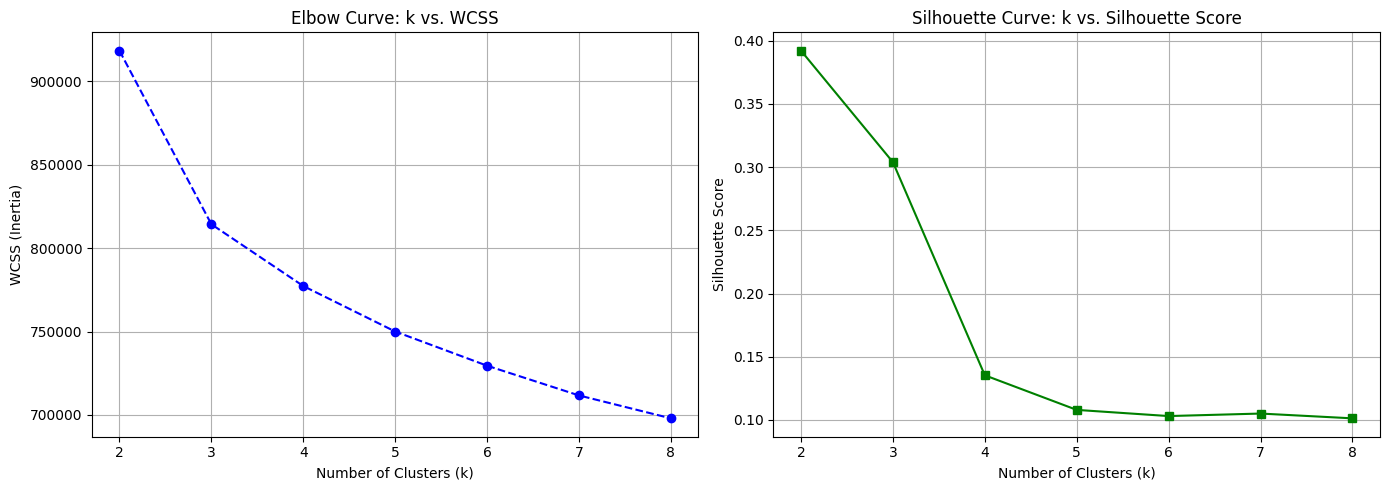
\includegraphics[width=0.65\linewidth]{elbow_sil.png}
    \caption{Elbow Curve and Silhouette Score used for selecting optimal k}
\end{figure}
\subsection*{DBSCAN}
- Density-based clustering algorithm.  
- Parameters: $\epsilon$ (neighborhood radius), $minPts$ (minimum points).  
- Core points, border points, and noise are identified.  
- Advantage: Can discover clusters of arbitrary shape and handle noise.

\subsection*{Hierarchical Clustering}
- Builds hierarchy of clusters using either:
\begin{itemize}
    \item Agglomerative (bottom-up merging).
    \item Divisive (top-down splitting).
\end{itemize}
- Linkage criteria: Single, Complete, Average, Ward’s method.  
- Represented by a dendrogram.

\section*{Clustering Implementation}

\textbf{Model A: K-Means} \\
Configured with k=6 using the k-means++ initialization method to ensure optimal centroid placement.

\vspace{0.3cm}

\textbf{Model B: DBSCAN} \\
Configured with an epsilon ($\epsilon$) neighborhood radius of 15.0 and minimum points ($\text{minPts}$) set to 10. These parameters were tuned to handle the high-dimensional sparsity of the HAR dataset.

\vspace{0.3cm}

\textbf{Model C: Hierarchical Agglomerative Clustering (HAC)} \\
Implemented using a bottom-up approach with $n\_clusters=6$, utilizing the Euclidean distance metric and Ward's linkage criterion to minimize within-cluster variance.
\begin{figure}[H]
    \centering
    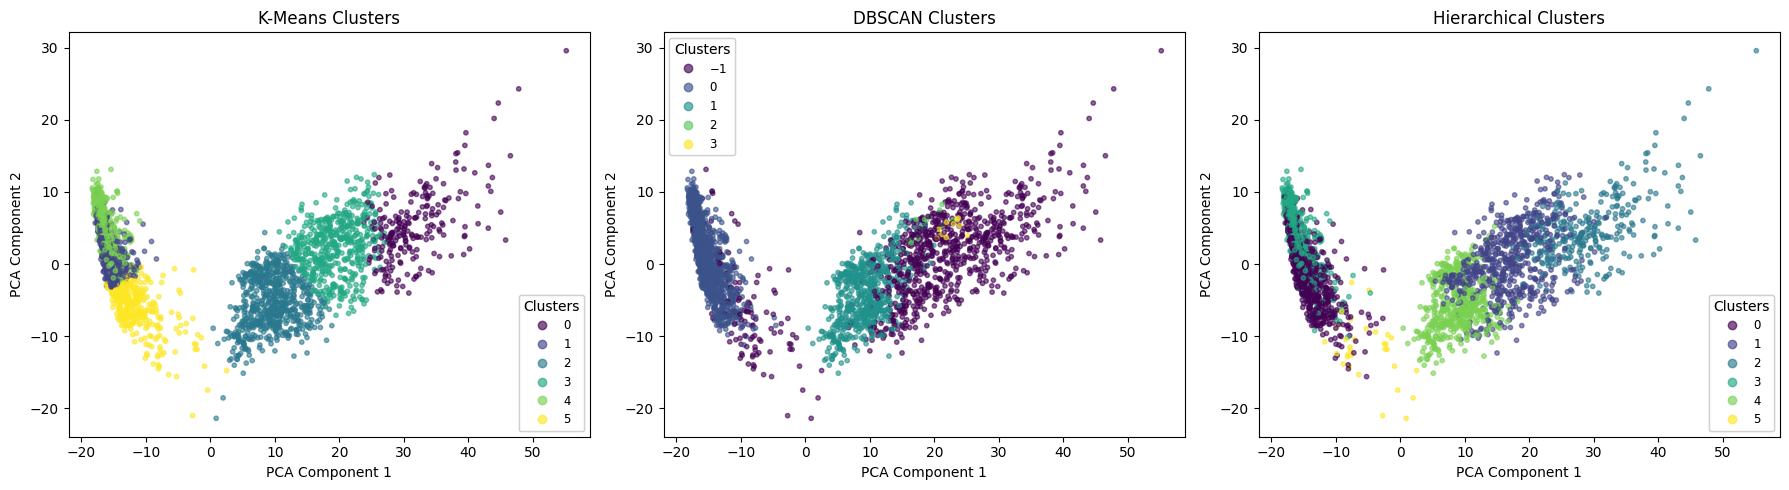
\includegraphics[width=0.65\linewidth]{pca2d.png}
    \caption{PCA 2D Visualization}
\end{figure}

\begin{figure}[H]
    \centering
    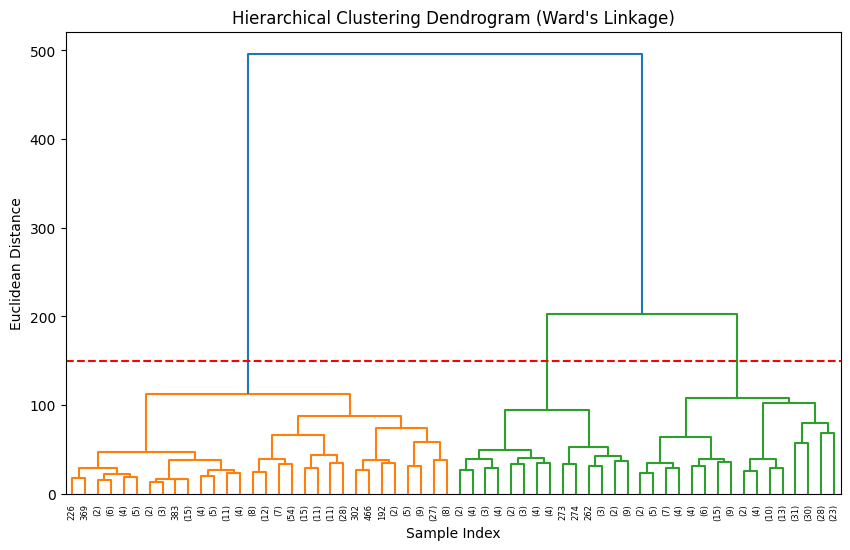
\includegraphics[width=0.65\linewidth]{dendogram.png}
    \caption{Dendrogram}
\end{figure}

\section*{Evaluation Metrics}
\begin{table}[H]
\centering
\caption{Clustering Evaluation Metrics}
\renewcommand{\arraystretch}{1.3}
\begin{tabularx}{\textwidth}{|X|X|X|X|X|X|}
\hline
\textbf{Algorithm} & \textbf{Silhouette} & \textbf{Davies-Bouldin} & \textbf{Calinski-Harabasz} & \textbf{ARI} & \textbf{NMI} \\
\hline
K-Means & 0.1030 & 2.6595 & 744.809 & 0.4344 & 0.5735 \\
DBSCAN & 0.1865 & 2.4866 & 563.785 & 0.2904 & 0.4362 \\
Hierarchical (Ward) & 0.0970 & 2.5856 & 705.173 & 0.5217 & 0.6417 \\
\hline
\end{tabularx}
\end{table}

\section*{Observations and Comparative Analysis}

\begin{enumerate}

\item \textbf{Which algorithm produced the most meaningful clusters? Why?} \\
Hierarchical Agglomerative Clustering (HAC) with Ward's linkage and K-Means produced the most meaningful clusters. Both algorithms successfully grouped the data into distinct segments that closely mapped to the actual physical activities (as evidenced by their higher NMI and ARI scores). Because the HAR dataset's true clusters (the 6 activities) are relatively globular and have comparable variances, algorithms that minimize intra-cluster variance (like K-Means and Ward's HAC) perform exceptionally well.

\item \textbf{How sensitive was K-Means to the choice of $k$?} \\
K-Means was highly sensitive to the chosen $k$. Selecting a $k$ lower than 6 forced the algorithm to merge distinct but similar activities (such as SITTING and STANDING, which have similar sensor profiles). Selecting a $k$ higher than 6 caused cohesive activity clusters (like WALKING) to be artificially split into arbitrary sub-clusters, significantly reducing the external evaluation scores.

\item \textbf{Did DBSCAN detect noise or small clusters effectively?} \\
DBSCAN struggled to form meaningful, distinct clusters on this specific dataset. In highly dimensional spaces (561 features), the ``curse of dimensionality'' causes the distances between all pairs of points to become relatively uniform. Consequently, DBSCAN either grouped the majority of the data into one massive continuous cluster or labeled a large portion of the dataset as noise, depending on slight tweaks to the $\epsilon$ parameter. While it detected outliers, it failed to isolate the 6 core activities effectively.

\item \textbf{How does linkage choice (single/complete/ward) affect hierarchical clustering?} \\
Linkage criteria fundamentally change the dendrogram structure. Single linkage (nearest neighbor) suffers severely from ``chaining,'' creating long, unhelpful clusters where almost all points attach to a single giant cluster one by one. Complete linkage (furthest neighbor) avoids chaining but is highly sensitive to outliers. Ward's linkage, which was used in this experiment, minimizes the total within-cluster variance at each merge step. This resulted in the most balanced, compact, and spherical clusters, which best represented the actual physical activities.

\item \textbf{Which internal metric best matched your visual intuition of cluster quality?} \\
The Davies-Bouldin (DB) Index and the Calinski-Harabasz (CH) Index matched visual intuition the best. When looking at the PCA scatter plots, K-Means and HAC showed tight, separated groupings. The DB index (which measures the ratio of within-cluster scatter to between-cluster separation) mathematically confirmed this by rewarding the models that formed these compact, distinct groupings. While the Silhouette score was useful, it tends to penalize overlapping clusters heavily, which is natural in the HAR dataset where static activities (Sitting/Standing) organically overlap in sensor space.

\end{enumerate}

\section*{Conclusion}

This experiment demonstrated the strengths and limitations of various clustering algorithms on high-dimensional sensor data. K-Means and Hierarchical Clustering with Ward's linkage proved highly effective for the HAR dataset because the underlying physical activities form relatively spherical, variance-bound groupings.

Evaluating these models required a combination of the Elbow method and internal metrics (Silhouette Score, Davies-Bouldin Index) to optimize parameters when ground truth is assumed hidden, alongside external metrics (Adjusted Rand Index (ARI), Normalized Mutual Information (NMI)) to validate the final groupings against the actual activity labels.

Conversely, density-based approaches like DBSCAN proved challenging to tune and less effective due to the sparsity inherent in high-dimensional Euclidean spaces.

\end{document}
